\documentclass[11pt,a4paper]{article}
\usepackage[T1]{fontenc}
\usepackage[utf8]{inputenc}
\usepackage[provide=*,italian]{babel}
\usepackage{lmodern,microtype,geometry}
\geometry{margin=2.5cm}
\usepackage{amsmath,amssymb,amsthm,mathtools}
\usepackage{booktabs,array,longtable}
\usepackage{xcolor,enumitem,tikz}
\usetikzlibrary{arrows.meta,positioning,calc}
\usepackage[most]{tcolorbox}
\usepackage{listings,hyperref,fancyhdr}

\definecolor{sapienzared}{RGB}{130,0,36}
\definecolor{softred}{RGB}{249,241,243}
\definecolor{softblue}{RGB}{239,246,252}
\definecolor{softgray}{RGB}{245,245,245}
\definecolor{codegreen}{RGB}{25,110,65}
\hypersetup{colorlinks=true,linkcolor=sapienzared,urlcolor=sapienzared,
pdftitle={Il simplesso su reti},pdfauthor={Giampaolo Liuzzi}}

\pagestyle{fancy}\fancyhf{}
\fancyhead[L]{\small Ottimizzazione su Reti}
\fancyhead[R]{\small Capitolo 5}
\fancyfoot[C]{\thepage}
\renewcommand{\headrulewidth}{0.4pt}

\newtheorem{definition}{Definizione}[section]
\newtheorem{theorem}[definition]{Teorema}
\newtheorem{proposition}[definition]{Proposizione}
\newtheorem{observation}[definition]{Osservazione}
\newtcolorbox{learningbox}{colback=softred,colframe=sapienzared,title=Obiettivi di apprendimento,fonttitle=\bfseries,boxrule=0.8pt,arc=1.5mm}
\newtcolorbox{examplebox}[1]{colback=softblue,colframe=blue!55!black,title=#1,fonttitle=\bfseries,boxrule=0.7pt,arc=1.5mm}
\newtcolorbox{notationbox}{colback=softgray,colframe=black!55,title=Registro delle notazioni,fonttitle=\bfseries,boxrule=0.7pt,arc=1.5mm}
\newtcolorbox{warningbox}{colback=yellow!9,colframe=orange!65!black,title=Attenzione,fonttitle=\bfseries,boxrule=0.7pt,arc=1.5mm}
\newtcolorbox{networkxbox}{colback=softgray,colframe=black!55,title=Python/NetworkX,fonttitle=\bfseries,boxrule=0.7pt,arc=1.5mm}
\lstdefinestyle{python}{language=Python,basicstyle=\ttfamily\small,keywordstyle=\color{blue!65!black}\bfseries,commentstyle=\color{codegreen},stringstyle=\color{sapienzared},backgroundcolor=\color{softgray},frame=single,rulecolor=\color{black!25},showstringspaces=false,breaklines=true,columns=fullflexible}

\newcommand{\V}{\mathcal{V}}
\newcommand{\E}{\mathcal{E}}
\newcommand{\R}{\mathbb{R}}
\newcommand{\Bset}{\mathcal{B}}
\newcommand{\Nset}{\mathcal{N}}
\newcommand{\Sset}{\mathcal{S}}

\begin{document}
\hypersetup{pageanchor=false}
\begin{titlepage}
\centering\vspace*{1.6cm}
{\color{sapienzared}\rule{\textwidth}{1.2pt}}\\[1.1cm]
{\Large Ottimizzazione su Reti}\\[0.35cm]
{\huge\bfseries Capitolo 5}\\[0.45cm]
{\LARGE\bfseries Il simplesso su reti}\\[1.1cm]
{\color{sapienzared}\rule{0.72\textwidth}{0.8pt}}\\[1.1cm]
{\large Corso di Laurea Magistrale in Ingegneria Gestionale}\\[0.25cm]
{\large Sapienza Università di Roma}\\[1.2cm]
{\large Giampaolo Liuzzi}\\[0.25cm]
{\normalsize Dipartimento di Ingegneria Informatica, Automatica e Gestionale}
\vfill{\small Versione preliminare per uso didattico}
\end{titlepage}
\hypersetup{pageanchor=true}
\pagenumbering{roman}\tableofcontents\newpage\pagenumbering{arabic}

\begin{learningbox}
Al termine del capitolo lo studente dovrebbe essere in grado di:
\begin{itemize}[nosep]
\item interpretare una soluzione di base mediante un albero ricoprente;
\item calcolare il flusso di base con eliminazioni successive delle foglie;
\item determinare potenziali e costi ridotti senza invertire matrici;
\item eseguire un'iterazione del simplesso mediante il ciclo fondamentale;
\item riconoscere ottimalità, illimitatezza e degenerazione;
\item trattare correttamente reti capacitate e ottenere una soluzione iniziale.
\end{itemize}
\end{learningbox}

\section{Il problema di flusso a costo minimo}

Consideriamo una rete orientata e connessa $G=(\V,\E)$, con costo $c_{ij}$ per ogni arco $(i,j)$ e domanda $b_i$ per ogni nodo. Manteniamo la convenzione dei capitoli precedenti:
\[
b_i>0\ \text{domanda},\qquad b_i<0\ \text{offerta},\qquad
A_{i,(h,k)}=\begin{cases}-1&i=h,\\+1&i=k,\\0&\text{altrimenti.}\end{cases}
\]
Il problema non capacitato è
\begin{equation}\label{eq:mcf}
\min\ c^\top x\qquad \text{s.t.}\qquad Ax=b,\quad x\geq0.
\end{equation}
Poiché le righe di $A$ sommano a zero, è necessario che $\sum_{i\in\V}b_i=0$. Se il grafo sottostante è connesso, $\operatorname{rank}(A)=n-1$: eliminiamo quindi una riga e lavoriamo con il sistema ridotto $\bar A x=\bar b$.

\section{Basi e alberi ricoprenti}

\begin{theorem}[Alberi e basi]
Un insieme di $n-1$ colonne di $\bar A$ forma una base se e solo se i corrispondenti archi, considerati senza orientamento, formano un albero ricoprente di $G$.
\end{theorem}

Indichiamo con $\Bset$ gli archi dell'albero e con $\Nset=\E\setminus\Bset$ gli archi fuori base. Nel caso non capacitato una soluzione di base si ottiene ponendo
\[
x_{\Nset}=0,\qquad x_{\Bset}=B^{-1}\bar b.
\]
Essa è ammissibile se $x_{\Bset}\geq0$. Dunque non ogni albero ricoprente determina necessariamente una soluzione di base \emph{ammissibile}.

\subsection{Calcolo del flusso per eliminazione delle foglie}

Non è necessario calcolare $B^{-1}$. Si sceglie una radice $r$ e si considera una foglia $v\neq r$ dell'albero corrente. Il solo arco di albero incidente a $v$ è $e$.
\begin{itemize}
\item Se $e=(u,v)$ entra in $v$, il bilancio impone $x_e=b_v$.
\item Se $e=(v,u)$ esce da $v$, il bilancio impone $x_e=-b_v$.
\end{itemize}
Si elimina $v$ e si trasferisce il suo bilancio al nodo $u$; ripetendo, si determinano tutti i flussi di albero. Un valore negativo segnala che la base non è ammissibile.

\begin{examplebox}{Un flusso di base}
Siano $b_1=-7$, $b_2=3$, $b_3=4$ e $\Bset=\{(1,2),(1,3)\}$. Dalle due foglie si ottiene
\[
x_{12}=3,\qquad x_{13}=4.
\]
Il bilancio del nodo 1 è $-3-4=-7$. La soluzione è ammissibile.
\end{examplebox}

\section{Duale, potenziali e costi ridotti}

Il duale di \eqref{eq:mcf} è
\[
\max\ b^\top y\qquad\text{s.t.}\qquad A^\top y\leq c.
\]
Per l'arco $(i,j)$, la disuguaglianza duale è
\[
y_j-y_i\leq c_{ij}.
\]
Le variabili $y_i$ sono dette \emph{potenziali dei nodi}. Il costo ridotto è
\begin{equation}\label{eq:ridotto}
\gamma_{ij}=c_{ij}-(y_j-y_i)=c_{ij}+y_i-y_j.
\end{equation}

Per gli archi di albero imponiamo $\gamma_{ij}=0$, cioè
\[
y_j-y_i=c_{ij}\qquad (i,j)\in\Bset.
\]
Fissato arbitrariamente il potenziale della radice, per esempio $y_r=0$, gli altri potenziali si calcolano percorrendo l'albero. Se un arco di albero è attraversato nel verso opposto al suo orientamento, il costo va sottratto.

\begin{proposition}[Condizione di ottimalità]
Una soluzione di base ammissibile del problema non capacitato è ottima se
\[
\gamma_{ij}\geq0\qquad\forall(i,j)\in\Nset.
\]
\end{proposition}

\begin{examplebox}{Calcolo dei potenziali}
Siano archi di albero $(1,2)$ di costo $2$ e $(3,2)$ di costo $1$. Posto $y_1=0$, si ha $y_2=2$ e, poiché $y_2-y_3=1$, $y_3=1$. Per un arco fuori base $(1,3)$ di costo $-1$,
\[
\gamma_{13}=-1+y_1-y_3=-2<0,
\]
quindi la soluzione corrente non è ottima.
\end{examplebox}

\section{Il pivot come ciclo fondamentale}

Sia $(p,q)\in\Nset$ un arco con $\gamma_{pq}<0$. Aumentare $x_{pq}$ riduce la funzione obiettivo. Aggiungendo $(p,q)$ all'albero si crea un unico ciclo. Lo percorriamo nel verso dell'arco entrante e partizioniamo gli archi in
\[
C^+=\{\text{archi percorsi concordemente}\},\qquad
C^-=\{\text{archi percorsi in verso discorde}\}.
\]
Per conservare i bilanci, aumentiamo di $\theta$ il flusso sugli archi di $C^+$ e lo diminuiamo sugli archi di $C^-$. Nel caso non capacitato,
\[
\theta=\min_{e\in C^-}x_e.
\]
Un arco che raggiunge flusso zero esce dalla base. Se $C^-=\varnothing$, il flusso può crescere indefinitamente e il problema è illimitato inferiormente.

\begin{figure}[ht]
\centering
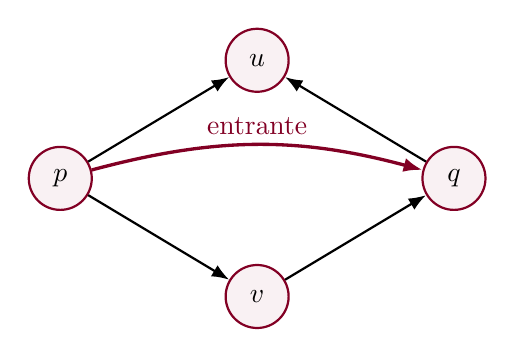
\begin{tikzpicture}[node/.style={circle,draw=sapienzared,thick,fill=softred,minimum size=8mm},arc/.style={-{Latex[length=2.2mm]},thick},enter/.style={-{Latex[length=2.4mm]},very thick,sapienzared}]
\node[node] (a) at (0,0) {$p$}; \node[node] (b) at (2.5,1.5) {$u$};
\node[node] (c) at (5,0) {$q$}; \node[node] (d) at (2.5,-1.5) {$v$};
\draw[arc] (a)--(b); \draw[arc] (c)--(b);
\draw[arc] (d)--(c); \draw[arc] (a)--(d);
\draw[enter,bend left=15] (a) to node[above] {entrante} (c);
\end{tikzpicture}
\caption{L'arco entrante chiude il ciclo fondamentale; alcuni archi sono percorsi concordemente e altri discordemente.}
\end{figure}

La variazione del costo lungo il ciclo è
\[
\Delta z=\theta\left(\sum_{e\in C^+}c_e-\sum_{e\in C^-}c_e\right)
=\theta\gamma_{pq}<0.
\]
Questa identità spiega geometricamente il ruolo del costo ridotto.

\section{Algoritmo per il caso non capacitato}

\begin{enumerate}
\item Partire da un albero $\Bset$ che definisca un flusso di base ammissibile.
\item Calcolare i potenziali imponendo $y_r=0$ e $\gamma_e=0$ per $e\in\Bset$.
\item Calcolare $\gamma_e$ per $e\in\Nset$. Se tutti sono non negativi, terminare.
\item Scegliere un arco entrante $e\in\Nset$ con $\gamma_e<0$.
\item Costruire il ciclo fondamentale e calcolare $\theta=\min_{a\in C^-}x_a$.
\item Se $C^-=\varnothing$, dichiarare il problema illimitato; altrimenti aggiornare i flussi.
\item Scegliere un arco uscente che raggiunge zero, aggiornare l'albero e tornare al passo 2.
\end{enumerate}

Una regola naturale sceglie l'arco con costo ridotto più negativo. In presenza di degenerazione, regole anticiclo come quella di Bland garantiscono terminazione finita.

\section{Reti capacitate}

Consideriamo ora
\begin{equation}\label{eq:cap}
\min\ c^\top x\qquad\text{s.t.}\qquad Ax=b,\quad 0\leq x\leq u.
\end{equation}
Una base ad albero induce una tripartizione:
\begin{itemize}
\item $\Bset$: archi di albero, con flusso determinato dai bilanci;
\item $\Nset$: archi fuori albero al limite inferiore, $x_e=0$;
\item $\Sset$: archi fuori albero saturi, $x_e=u_e$.
\end{itemize}
Il flusso sugli archi di albero soddisfa
\[
B x_{\Bset}=\bar b-Su_{\Sset}.
\]

\begin{theorem}[Ottimalità nel caso capacitato]
Una soluzione di base ammissibile è ottima se
\[
\gamma_e\geq0\quad\forall e\in\Nset,
\qquad
\gamma_e\leq0\quad\forall e\in\Sset.
\]
\end{theorem}

Un arco vuoto con $\gamma_e<0$ può entrare aumentando il proprio flusso. Un arco saturo con $\gamma_e>0$ può entrare diminuendolo. Nel secondo caso è utile pensare all'arco residuo inverso, di capacità $u_e-x_e$ e costo $-c_e$.

\subsection{Calcolo del passo}

Se entra un arco vuoto, il ciclo è percorso nel verso dell'arco entrante e
\[
\theta=\min\left\{
\min_{e\in C^+}(u_e-x_e),
\min_{e\in C^-}x_e
\right\}.
\]
Se entra un arco saturo, se ne diminuisce il flusso; equivalentemente si percorre il ciclo nel verso opposto e si applica la stessa regola residua. Il passo termina quando un arco raggiunge zero o capacità. L'arco bloccante esce dall'albero; l'arco entrante può anche raggiungere il limite opposto senza entrare stabilmente in base.

\begin{warningbox}
Nel caso capacitato non basta controllare i costi ridotti degli archi vuoti. Anche un arco saturo con costo ridotto positivo viola l'ottimalità, perché ridurne il flusso può diminuire il costo totale.
\end{warningbox}

\section{Degenerazione e scelte multiple}

Un pivot è \emph{degenere} se $\theta=0$. L'albero cambia ma il flusso e il valore della funzione obiettivo restano invariati. La degenerazione può verificarsi quando un arco di albero è già a un limite oppure più archi diventano bloccanti simultaneamente.

Se più archi possono uscire, si deve sceglierne uno preservando la struttura di albero. Se più costi ridotti violano l'ottimalità, diverse regole di ingresso producono percorsi algoritmici diversi ma non modificano le condizioni di correttezza.

\section{Ricerca di una soluzione iniziale}

L'ipotesi di disporre di una base ammissibile non è sempre realistica. Una procedura generale introduce un nodo artificiale $0$ e archi artificiali che consentono di soddisfare i bilanci:
\begin{itemize}
\item per $b_i>0$, si introduce $(0,i)$;
\item per $b_i<0$, si introduce $(i,0)$.
\end{itemize}
Agli archi artificiali si assegna un costo $M$ sufficientemente grande, oppure si minimizza in una Fase I la somma dei loro flussi. Gli archi artificiali formano inizialmente un albero a stella e forniscono una soluzione ammissibile del problema ausiliario.

Se all'ottimo della Fase I rimane flusso artificiale positivo, il problema originario è inammissibile. Altrimenti gli archi artificiali possono essere eliminati e si passa alla minimizzazione dei costi originali.

\section{Un'iterazione completa}

Consideriamo $\V=\{1,2,3,4\}$, $b=(-5,0,2,3)$ e gli archi riportati in tabella.
\begin{center}
\begin{tabular}{cccccc}
\toprule
Arco & $(1,2)$ & $(2,3)$ & $(2,4)$ & $(1,3)$ & $(3,4)$\\
Costo & $2$ & $2$ & $4$ & $1$ & $1$\\
\bottomrule
\end{tabular}
\end{center}
Sia $\Bset=\{(1,2),(2,3),(2,4)\}$. Dalle foglie $3$ e $4$ si ricava
\[
x_{23}=2,\qquad x_{24}=3,\qquad x_{12}=5,
\]
con costo $5\cdot2+2\cdot2+3\cdot4=26$. Posto $y_1=0$, le uguaglianze sugli archi di albero danno
\[
y_2=2,qquad y_3=4,qquad y_4=6.
\]
Per l'arco $(1,3)$,
\[
\gamma_{13}=1+y_1-y_3=-3,
\]
che entra. Il ciclo è $1\to3\leftarrow2\leftarrow1$: aumentano $x_{13}$ e diminuiscono $x_{23}$ e $x_{12}$. Pertanto
\[
\theta=\min\{x_{23},x_{12}\}=2.
\]
Esce $(2,3)$ e il nuovo flusso è $x_{13}=2$, $x_{12}=3$, $x_{24}=3$, con costo $20$.

\section{Python e NetworkX}

\begin{networkxbox}
NetworkX implementa il flusso a costo minimo mediante \texttt{network\_simplex}. Con la nostra convenzione il valore \texttt{demand} coincide direttamente con $b_i$: positivo per domanda e negativo per offerta. Non occorre cambiare segno.
\end{networkxbox}

\begin{lstlisting}[style=python,caption={Soluzione del problema dell'esempio con NetworkX}]
import networkx as nx

G = nx.DiGraph()
for i, b in {1: -5, 2: 0, 3: 2, 4: 3}.items():
    G.add_node(i, demand=b)

arcs = [
    (1, 2, 2), (2, 3, 2), (2, 4, 4),
    (1, 3, 1), (3, 4, 1)
]
for i, j, c in arcs:
    G.add_edge(i, j, weight=c, capacity=10)

cost, flow = nx.network_simplex(G)
print(cost)
for i, j in G.edges:
    print((i, j), flow[i][j])
\end{lstlisting}

NetworkX restituisce una soluzione ottima, ma non espone direttamente l'albero di base, i potenziali o i pivot. Per finalità didattiche è quindi utile implementare separatamente le singole operazioni: calcolo dei flussi sull'albero, potenziali, costi ridotti e ciclo fondamentale.

\section{Registro delle notazioni}

\begin{notationbox}
\begin{center}
\begin{tabular}{ll}
\toprule
Simbolo & Significato\\
\midrule
$A,\bar A$ & matrice di incidenza e matrice ridotta\\
$b_i$ & domanda se positiva, offerta se negativa\\
$\Bset$ & archi dell'albero di base\\
$\Nset$ & archi fuori base al limite inferiore\\
$\Sset$ & archi fuori base saturi\\
$y_i$ & potenziale del nodo $i$\\
$\gamma_{ij}$ & $c_{ij}+y_i-y_j$, costo ridotto\\
$C^+,C^-$ & archi concordi e discordi nel ciclo\\
$u_{ij}$ & capacità dell'arco $(i,j)$\\
$\theta$ & ampiezza del pivot\\
\bottomrule
\end{tabular}
\end{center}
\end{notationbox}

\section{Errori frequenti}
\begin{enumerate}
\item Usare $b_i>0$ per un'offerta: qui, come in NetworkX, indica una domanda.
\item Dimenticare che una base è una matrice ridotta di ordine $n-1$.
\item Ritenere ammissibile ogni albero ricoprente senza controllare i flussi.
\item Calcolare $\gamma_{ij}$ con il segno opposto: qui $\gamma_{ij}=c_{ij}+y_i-y_j$.
\item Aggiornare tutti gli archi del ciclo nello stesso verso.
\item Nel caso capacitato, controllare soltanto gli archi vuoti.
\item Confondere arco entrante nell'albero e aumento del flusso: per un arco saturo il flusso diminuisce.
\item Interpretare un pivot degenere come arresto dell'algoritmo.
\end{enumerate}

\section{Esercizi}

\textbf{Esercizio 5.1 -- Flusso di base.}
Dato un albero orientato, scegliere una radice e calcolare i flussi per eliminazione delle foglie. Verificare i bilanci $Ax=b$.

\medskip\textbf{Esercizio 5.2 -- Potenziali.}
Per la base dell'Esercizio 5.1 porre $y_r=0$, calcolare i potenziali e tutti i costi ridotti. Stabilire se la soluzione è ottima.

\medskip\textbf{Esercizio 5.3 -- Pivot.}
Scegliere un arco con costo ridotto negativo, costruire il ciclo fondamentale, determinare $C^+$, $C^-$, $\theta$ e il nuovo albero.

\medskip\textbf{Esercizio 5.4 -- Capacità.}
Ripetere l'Esercizio 5.3 introducendo capacità finite. Individuare l'arco bloccante e classificare gli archi nei tre insiemi $\Bset$, $\Nset$, $\Sset$.

\medskip\textbf{Esercizio 5.5 -- Fase I.}
Costruire la rete artificiale per un'istanza con due nodi di offerta e tre di domanda e scrivere la soluzione iniziale a stella.

\medskip\textbf{Esercizio 5.6 -- NetworkX.}
Implementare l'esempio completo, verificare costo e bilanci, quindi modificare una capacità in modo da cambiare la soluzione ottima.

\section{Sintesi del capitolo}
\begin{learningbox}
\begin{itemize}[nosep]
\item Le basi della matrice di incidenza ridotta corrispondono agli alberi ricoprenti.
\item Flussi e potenziali si calcolano percorrendo l'albero, senza inversioni di matrici.
\item Un costo ridotto violato individua un arco entrante e crea un ciclo fondamentale.
\item Il test del rapporto è sostituito dal primo limite di flusso raggiunto lungo il ciclo.
\item Nelle reti capacitate gli archi fuori albero sono vuoti o saturi.
\item La convenzione $Ax=b$ coincide con l'attributo \texttt{demand} di NetworkX.
\end{itemize}
\end{learningbox}

\paragraph{Verso i capitoli successivi.}
Il flusso massimo e il cammino minimo saranno ricavati come casi particolari del flusso a costo minimo. Potenziali, costi ridotti e rete residua riappariranno con interpretazioni specifiche.

\end{document}
